\begin{figure} [H]
	\begin{center}
		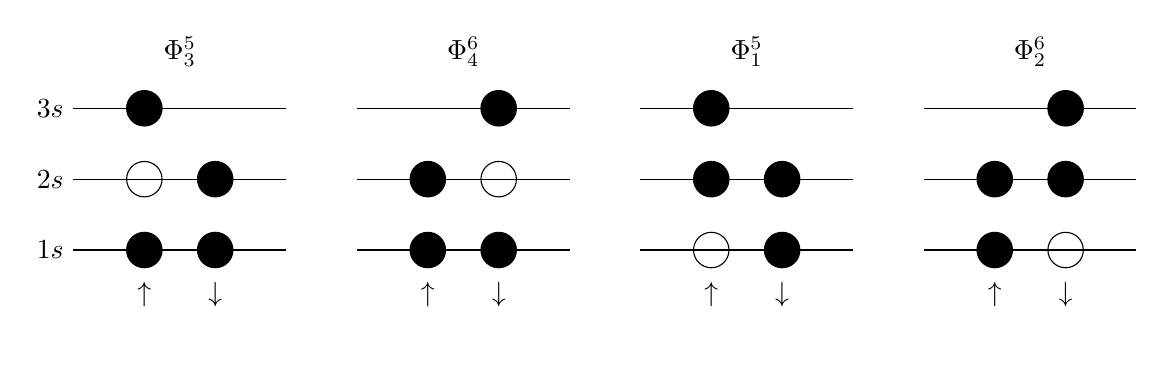
\begin{tikzpicture}[scale=0.9]
		\begin{scope}
		\foreach \i in {1,...,3}
		{
			\draw (-1,\i-1) node[anchor=east] {$\i s$} --(2,\i-1);
		}
		\filldraw (0,0) node[anchor=north,inner sep=.4cm] {$\uparrow$} circle (0.25cm); 
		\filldraw (1,0) node[anchor=north,inner sep=.4cm] {$\downarrow$} circle (0.25cm);
		\draw (0,1) circle (0.25cm);
		\filldraw (1,1) circle (0.25cm);
		\filldraw (0,2) circle (0.25cm);
		\node[] at (0.5,2.8) {$\ket{\Phi_3^5}$};
		\end{scope}
		\begin{scope}[xshift=4cm]
		\foreach \i in {1,...,3}
		{
			\draw (-1,\i-1) --(2,\i-1);
		}
		\filldraw (0,0) node[anchor=north,inner sep=.4cm] {$\uparrow$} circle (0.25cm); 
		\filldraw (1,0) node[anchor=north,inner sep=.4cm] {$\downarrow$} circle (0.25cm);
		\draw (1,1) circle (0.25cm);
		\filldraw (1,2) circle (0.25cm);
		\filldraw (0,1) circle (0.25cm);
		\node[] at (0.5,2.8) {$\ket{\Phi_{4}^{6}}$};
		\end{scope}
		\begin{scope}[xshift=8cm]
		\foreach \i in {1,...,3}
		{
			\draw (-1,\i-1) -- (2,\i-1);
		}
		\draw (0,0) node[anchor=north,inner sep=.4cm] {$\uparrow$} circle (0.25cm); 
		\filldraw (1,0) node[anchor=north,inner sep=.4cm] {$\downarrow$} circle (0.25cm);
		\filldraw (0,1) circle (0.25cm);
		\filldraw (1,1) circle (0.25cm);
		\filldraw (0,2) circle (0.25cm);
		\node[] at (0.5,2.8) {$\ket{\Phi_{1}^{5}}$};
		\end{scope}
		\begin{scope}[xshift=12cm]
		\foreach \i in {1,...,3}
		{
			\draw (-1,\i-1) --(2,\i-1);
		}
		\filldraw (0,0) node[anchor=north,inner sep=.4cm] {$\uparrow$} circle (0.25cm); 
		\draw (1,0) node[anchor=north,inner sep=.4cm] {$\downarrow$} circle (0.25cm);
		\filldraw (1,1) circle (0.25cm);
		\filldraw (1,2) circle (0.25cm);
		\filldraw (0,1) circle (0.25cm);
		\node[] at (0.5,2.8) {$\ket{\Phi_{2}^{6}}$};
		\end{scope}
		\end{tikzpicture}
	\end{center}
	\newline
	\begin{center}
		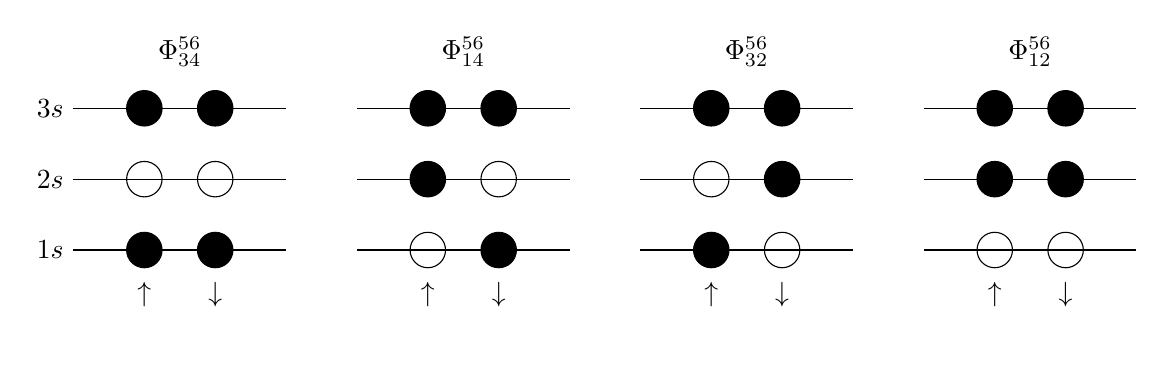
\begin{tikzpicture}[scale=0.9]
		\begin{scope}
		\foreach \i in {1,...,3}
		{
			\draw (-1,\i-1) node[anchor=east] {$\i s$} --(2,\i-1);
		}
		\filldraw (0,0) node[anchor=north,inner sep=.4cm] {$\uparrow$} circle (0.25cm); 
		\filldraw (1,0) node[anchor=north,inner sep=.4cm] {$\downarrow$} circle (0.25cm);
		\draw (0,1) circle (0.25cm);
		\draw (1,1) circle (0.25cm);
		\filldraw (0,2) circle (0.25cm);
		\filldraw (1,2) circle (0.25cm);
		\node[] at (0.5,2.8) {$\ket{\Phi_{34}^{56}}$};
		\end{scope}
		\begin{scope}[xshift=4cm]
		\foreach \i in {1,...,3}
		{
			\draw (-1,\i-1) --(2,\i-1);
		}
		\draw (0,0) node[anchor=north,inner sep=.4cm] {$\uparrow$} circle (0.25cm); 
		\filldraw (1,0) node[anchor=north,inner sep=.4cm] {$\downarrow$} circle (0.25cm);
		\draw (1,1) circle (0.25cm);
		\filldraw (1,2) circle (0.25cm);
		\filldraw (0,2) circle (0.25cm);
		\filldraw (0,1) circle (0.25cm);
		\node[] at (0.5,2.8) {$\ket{\Phi_{14}^{56}}$};
		\end{scope}
		\begin{scope}[xshift=8cm]
		\foreach \i in {1,...,3}
		{
			\draw (-1,\i-1) -- (2,\i-1);
		}
		\filldraw (0,0) node[anchor=north,inner sep=.4cm] {$\uparrow$} circle (0.25cm); 
		\draw (1,0) node[anchor=north,inner sep=.4cm] {$\downarrow$} circle (0.25cm);
		\draw (0,1) circle (0.25cm);
		\filldraw (1,1) circle (0.25cm);
		\filldraw (0,2) circle (0.25cm);
		\filldraw (1,2) circle (0.25cm);
		\node[] at (0.5,2.8) {$\ket{\Phi_{32}^{56}}$};
		\end{scope}
		\begin{scope}[xshift=12cm]
		\foreach \i in {1,...,3}
		{
			\draw (-1,\i-1) --(2,\i-1);
		}
		\draw (0,0) node[anchor=north,inner sep=.4cm] {$\uparrow$} circle (0.25cm); 
		\draw (1,0) node[anchor=north,inner sep=.4cm] {$\downarrow$} circle (0.25cm);
		\filldraw (1,1) circle (0.25cm);
		\filldraw (1,2) circle (0.25cm);
		\filldraw (0,1) circle (0.25cm);
		\filldraw (0,2) circle (0.25cm);
		\node[] at (0.5,2.8) {$\ket{\Phi_{12}^{56}}$};
		\end{scope}
		\end{tikzpicture}
	\end{center}
	\caption{Possible states in the 1s, 2s and 3s orbitals of Beryllium. In the first row, all singly excited states are listed, while in the second row all doubly excited states are listed.}
	\label{fig:schematic}
\end{figure}